\newcommand{\strentD}[1]{\ensuremath{\rightsquigarrow^D}}
\newcommand{\FlatPR}{\textbf{FlatPR}}

\chapter{Reducing PR to Binary PR}\label{chap:pr_bpr}
In this chapter, we reduce \PR{} instances over an arbitrary finite alphabet $\Sigma : \finType$ to a binary alphabet over type $\bool$. The idea of this reduction is to replace every symbol $\sigma : \Sigma$ with a unique bitstring of length $\length{\Sigma}$. 
Thus, initial strings, rewrite windows, and final substrings need to be adapted.
This operation is incorporated using special string homomorphisms which we call uniform.

For the reduction, we need to modify the offset $o$ of the \PR{} instance by multiplying it with $\length{\Sigma}$\footnote{In fact, this reduction is the motivation for having the offset in the first place.}. This is motivated by the fact that, semantically, a bitstring of length $\length{\Sigma}$ represents a single symbol of the original alphabet.

The variant of \PR{} in which the alphabet is fixed to $\bool$ is called \BPR{}. All definitions of Section~\ref{sec:pr} carry over.

\section{Uniform Homomorphisms}
We introduce string homomorphisms and a special subclass of them, uniform homomorphisms.
While one usually uses string homomorphisms over a finite alphabet, we do not require finiteness for most of the definitions and results in this section.

\newcommand{\homomorphism}{\textsf{homomorphism}}
\begin{definition}[String Homomorphisms]
  Given types $\Sigma_1, \Sigma_2$, $h : \str{\Sigma_1} \rightarrow \str{\Sigma_2}$ is a homomorphism, written \mnotec{$\homomorphism~h$}, if $h (a_1 \concat a_2) = h~a_1 \concat h~a_2$ for all $a_1, a_2 : \str{\Sigma_1}$. 
\end{definition}

\begin{fact}
  Fix a homomorphism $h : \str{\Sigma_1} \rightarrow \str{\Sigma_2}$. 
  \begin{enumerate}
    \item $h~\nil = \nil$
    \item $h (a :: b) = h [a] \concat h~b$
    \item $h (\rconcat~l) = \rconcat~\withl h~x \withm x \in l \withr$
  \end{enumerate}
\end{fact}

\newcommand{\canonicalHom}{\textsf{canonicalHom}}
Given a function $f : \Sigma_1 \rightarrow \str{\Sigma_2}$, we can define a canonical homomorphism \[\canonicalHom~f \defeq \lambda~l. \rconcat~\withl f~x \withm x \in l \withr \mnote{\canonicalHom}\]  lifting $f$ to lists.

\begin{proposition}
  Let $f : \Sigma_1 \rightarrow \str{\Sigma_2}$. 
  \begin{enumerate}
    \item $\homomorphism~(\canonicalHom~f)$
    \item $\forall h, \homomorphism~h \rightarrow (\forall x, h [x] = f~x) \rightarrow h \equiv \canonicalHom~f$
  \end{enumerate}
\end{proposition}

A uniform homomorphism is a special kind of homomorphism. First of all, it is \emph{$\varepsilon$-free}, meaning that it only maps $\nil$ to $\nil$. Secondly, it maps all pairs of strings $a, b$ with $\length{a} = \length{b}$ to strings of the same length. 
Put differently, the length of every string is multiplied by a constant $k$ when passing through the homomorphism. 

\newcommand{\uniformHomo}{\textsf{uniformHom}}
\begin{definition}[Uniform Homomorphisms]
  \mnote{\uniformHomo}
  \[\uniformHomo~h \defeq \homomorphism~h \land (\forall x, \length{h~[x]} \ge 1) \land (\forall x_1~x_2, \length{h~[x_1]} = \length{h~[x_2]})\]
\end{definition}
Note that the definition is in terms of singleton lists. The more general property follows directly by using the properties of a homomorphism:
\begin{proposition}
  Let $h : \str{\Sigma_1} \rightarrow \str{\Sigma_2}$ with $\uniformHomo~h$.
  \begin{enumerate}
    \item $\length{l_1} = \length{l_2} \rightarrow \length{h~l_1} = \length{h~l_2}$
    \item $h~l = \nil \rightarrow l = \nil$
  \end{enumerate}
\end{proposition}

Again, we can define a canonical uniform homomorphism starting from a function $f : \Sigma_1 \rightarrow \str{\Sigma_2}$ satisfying $\length{f~x} = k > 0$ for all $x : \Sigma_1$. 
\begin{proposition}[Canonical Uniform Homomorphisms]
  Let $f : \Sigma_1 \rightarrow \str{\Sigma_2}$ with $\forall x, \length{f~x} = k$ for some $k > 0$. 
  Then $\uniformHomo~(\canonicalHom~f)$. 
\end{proposition}

Conversely, we can formalise the above intuition that the length of a string is multiplied by a constant $k$ when a uniform homomorphism is applied to it.
\begin{lemma}
  If $\Sigma : \finType$ and $\uniformHomo~h$, then $\sigtype{k}. \forall x, \length{h~x} = k \cdot \length{x}$. 
\end{lemma}
\begin{proof}
  As $\Sigma$ is a finite type, inhabitation is decidable. If $\length{\Sigma} = 0$, then we pick 42. 
  Otherwise, let $\sigma : \Sigma$ and pick $\length{h~[\sigma]}$. 
  For arbitrary $x : \str{\Sigma}$, the statement follows by induction on $x$ and using the defining properties of a uniform homomorphism.
\end{proof}

\section{Applying Uniform Homomorphisms to PR}\label{sec:unif_hom_pr}
We can show that \PR{} is invariant under injective uniform homomorphisms. That is, given a uniform homomorphism $h$ and a \PR{} instance $S$, we can define another \PR{} instance $S'$ where we have applied $h$ to all strings of $S$. $S'$ is a yes-instance if, and only if, $S$ is a yes-instance. 

Fix a \PR{} instance $S = (\Sigma_1, o, \omega, x_0, R, \Rfinal, t)$. 
Assume that $\length{\Sigma_1} > 0$. Instances of \PR{} not satisfying this property are trivial no-instances. 

Without loss of generality\footnote{This follows from the results of the previous section.}, we assume that the homomorphism is given as $h' : \Sigma_1 \rightarrow \Sigma_2$ with 
\begin{gather*}
  (A_1) \quad \length{h'~x} = k~\text{for a fixed } k > 0 \\
  (A_2) \quad \textsf{injective}~h'
\end{gather*}

Then define the full homomorphism $h \defeq \canonicalHom~h'$. 
Properties $(A_1)$ and $(A_2)$ carry over to $h$:
\begin{proposition}\label{prop:h_properties}\leavevmode
  \begin{enumerate}
    \item $\uniformHomo~h$
    \item $\length{h~x} = k \cdot \length{x}$
    \item $\textsf{injective}~h$
  \end{enumerate}
\end{proposition}

The following lemma allows us to split the image of $h$ along multiples of $k$ and follows from the properties of uniform homomorphisms in a straightforward way.
\begin{lemma}[Inversion of $h$]\label{lem:h_inv}\leavevmode
  \begin{enumerate}
    \item $h~a = u \concat v \rightarrow \length{u} = k \rightarrow \exists a_1~a_2, a = a_1 :: a_2 \land h~[a_1] = u \land h~a_2 = v$
    \item $h~a = u \concat v \rightarrow \length{u} = c \cdot k \rightarrow \exists a_1~a_2, a = a_1 \concat a_2 \land h~a_1 = u \land h~a_2 = v$ 
  \end{enumerate}
\end{lemma}

Homomorphisms can, of course, be lifted to rewrite windows. 
\begin{definition}
  \mnote{$h_{\text{window}}$}
  $h_\text{window}~w\defeq (h~(\prem w), h~(\conc~w)) $
\end{definition}
The transformed \PR{} instance is defined as
\begin{align*}
  \mnote{$R_h$}
  R_h &\defeq \withl h_\text{window}~w \withm w \in R \withr \\
  S' &\defeq (\Sigma_2, k \cdot o, k \cdot \omega, h~x_0, R_h, \withl h~l \withm l \in \Rfinal \withr, t).
  \mnote{$S'$}
\end{align*}
Note that the offset and the width both need to be multiplied by the multiplicative factor $k$ of $h$.
It is easy to see that this definition is well-formed, that is, $S'$ does again satisfy the syntactic constraints of \PR{} (Definition~\ref{def:pr}).
The goal for the rest of this section is to show that $\PR{}~S \leftrightarrow \PR{}~s'$. 

We start with the agreement of $\textsf{rewHead}$.
The first statement of the following lemma is the equivalence one would expect. However, it is rather weak, as the backwards direction requires that we know the premise and conclusion to be in the image of $h$.
For the proof of equivalence of $S$ and $S'$, we need a stronger statement: if we have a string $h~a$ that rewrites to a string $s$, we need to be able to derive that $s$ is in the image of $h$.

\begin{lemma}[Agreement of $\textsf{rewHead}$]\label{lem:rewHead_agree}\leavevmode
  \begin{enumerate}
    \item $\rewHead{w}{a}{b} \leftrightarrow \rewHead{(h_{\text{window}}~w)}{(h~a)}{(h~b)}$
    \item If $w \in \textsf{hwindows}$, $\length{a_1} = o$, $\length{u} = k \cdot o$, and $\rewHead{w}{(h~a_1 \concat h~a_2)}{(u \concat v)}$, then there exists $b_1$ with $u = h~b_1$ and $\length{b_1} = o$.
  \end{enumerate}
\end{lemma}
\begin{proof}
  Using Lemma~\ref{lem:h_inv} and the results of Proposition~\ref{prop:h_properties}.
\end{proof}

This can be lifted to $\strent{}$. For the proof, yet another characterisation of validity will be quite convenient:
\begin{gather*}
  \infer{a \strentD{R} b}{\length{a} = \length{b} \quad \length{a} = \omega \quad w \in R}
  \mnote{$\strentD{R}$}\\
  \infer{(u \concat a) \strentD{R} (v \concat b)}{a \strentD{R} b \quad \length{u} = o \quad \length{v} = o \quad w \in R \quad \rewHead{w}{(u \concat a)}{(v \concat b)}}
\end{gather*}
To some extent, this is the most intuitive characterisation of validity: it does not allow vacuous rewrites (i.e.\ allows only rewrites of length $\ge \omega$). Accordingly, it is not fully equivalent to $\strent{}$:
\begin{lemma}[Agreement of $\strent{}$ and $\strentD{}$]
  $a \strent{R} b \land \length{a} \ge \omega \leftrightarrow a \strentD{R} b$
\end{lemma}

The restriction to strings of length at least $\omega$ does not pose a problem as Definition~\ref{def:pr} imposes that as a syntactic constraint.
Using the new characterisation, we can now prove the equivalence for $\strent{}$.
\begin{lemma}[Agreement of $\strent{}$]
  Let $a$ with $\length{a} \ge \omega$ be given.
  \begin{enumerate}
    \item $(h~a) \strent{R_h} b' \rightarrow \exists b, b' = h~b \land a \strent{R} b$. 
    \item $a \strent{R} b \leftrightarrow (h~a) \strent{R_h} (h~b)$
  \end{enumerate}
\end{lemma}
\begin{proof}
  \begin{enumerate}
    \item We switch to $\strentD{}$ and do an induction on $\strentD{}$. In the base case, we show that the whole string is covered by the rewrite window and use the definition of $R_h$ and Lemma~\ref{lem:rewHead_agree}.1, as well as the facts provided by Proposition~\ref{prop:h_properties} and Lemma~\ref{lem:h_inv}.
      In the successor case, we use Lemma~\ref{lem:rewHead_agree}.2.
    \item Direction $\rightarrow$ follows by an easy induction. The other direction follows from 1.
  \end{enumerate}
\end{proof}

The equivalence trivially transfers to $\strent{}^n$: 
\begin{proposition}[Agreement of $\strent{}^n$]
  Let $a$ with $\length{a} \ge \omega$ be given.
  \begin{enumerate}
    \item $(h~a) \strent{R}^n b' \rightarrow \exists b, b' = h~b \land a \strent{R}^n b$
    \item $a \strent{R}^n b \leftrightarrow (h~a) \strent{R}^n (h~b)$
\end{enumerate}
\end{proposition}

%Finally, it needs to be shown that the final constraints agree:
%\begin{lemma}[Agreement of the Final Constraints]
  %Let $x_t$ with $\length{x_t} = \length{x_0}$ be given. Then 
  %\[x_t \models \Rfinal \leftrightarrow h~x_t \models \withl h~l \withm l \in \Rfinal \withr. \]
%\end{lemma}

After having show that the final constraints agree in the expected way, we can obtain the main agreement result.
\begin{theorem}\label{thm:hom_pr_equiv}
  $\PR{}~S \leftrightarrow \PR{}~S'$
\end{theorem}
%Thus, the transformed \PR{} instance is equivalent to the original instance.

\section{Reduction to \BPR{}}
The previous section's results can be applied to an injective uniform homomorphism into $\bool$ to directly obtain the reduction of \PR{} to \BPR{}. 
We use a homomorphism which just computes a unary encoding of the alphabet's elements over a binary alphabet. The $i$-th element $\sigma_i$ (counting from zero) of the finite type $\Sigma$ is mapped to the string $0^i10^{\length{\Sigma}-i-1}$.

Formally, let us fix a $\PR{}$-instance $S = (\Sigma, o, \omega, x_0, R, \Rfinal, t)$. In order to apply the results of the previous section, we rely on $\length{\Sigma} > 0$. We handle the case $\length{\Sigma} = 0$ separately in the end.

The following function defines the homomorphism for single elements. 
\begin{definition}\label{def:hnat_hsig}
  \begin{align*}
    \mnote{$h_{\nat}$}
    h_{\nat}~sig~n&\defeq \ITE{n~\overset{?}{<}~sig}{\bfalse^n \concat [\btrue] \concat \bfalse^{sig -n -1}}{\bfalse^{sig}} \\
    h_{\Sigma}~\sigma : \listsof{\bool} &\defeq h_{\nat}~(\length{\Sigma})~(\textsf{index}~\sigma)\mnote{$h_\Sigma$}
  \end{align*}
\end{definition}
The corresponding homomorphism can be obtained by using $\canonicalHom$. However, the technique of Section~\ref{sec:unif_hom_pr} justs asks us to provide a function operating on single symbols.

Properties $(A_1)$ and $(A_2)$ are straightforward to verify.

\begin{fact}[Uniformity]\leavevmode
  \begin{enumerate}
    \item $\length{h_{\nat}}~sig~n = sig$
    \item $\length{h_{\Sigma}~\sigma} = \length{\Sigma}$
  \end{enumerate}
\end{fact}

\begin{fact}[Injectivity]\leavevmode
  \begin{enumerate}
    \item $h_{\nat}~sig~m = \bfalse^n \concat [\btrue] \concat \bfalse^{sig - n - 1} \rightarrow m = n$
    \item $\textsf{injective}~h_{\Sigma}$
  \end{enumerate}
\end{fact}

The reduction now directly follows by Theorem~\ref{thm:hom_pr_equiv}.
In the special case of $\length{\Sigma} = 0$, the reduction maps to a trivial no-instance of \BPR{}. 

\begin{lemma}[\PR{} Reduces to \BPR{}]
  $\PR{}~S \leftrightarrow \BPR{}~S'$,
  where $S'$ is defined as in Section~\ref{sec:unif_hom_pr}.
\end{lemma}

\section{Mechanisation}
We briefly comment on the differences of the Coq mechanisation and the proof on paper as well as on the proof of computability. 

First of all, \BPR{} is defined to be a syntactically different problem from \PR{} in the Coq mechanisation. The only change is that the alphabet is fixed to $\bool$. Nearly all definitions (for instance the definition of $\strent{}$) can be re-used and do not need to be stated explicitly again.

Remember that we enforce the syntactic constraints on valid \PR{} instances (cf.\ Definition~\ref{def:pr}) externally. Therefore, we explicitly need to assume wellformedness of the \PR{} instance for the results of Section~\ref{sec:unif_hom_pr}. As wellformedness can be decided, the reduction maps non-wellformed instances to a trivial no-instance.

\BPR{} has the nice property of being directly extractable as we do not work over a general finite type anymore. Thus, it is not required to define a flat version of the problem again. However, as \PR{} still needs a separate flat version, our reduction structure looks as follows:
\begin{center}
  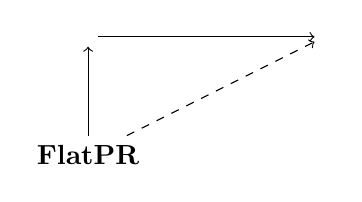
\begin{tikzpicture}
    \node (pr) at (0, 0) {\PR{}};
    \node (fpr) at (0, -1.5){\FlatPR{}};
    \node (bpr) at (3, 0) {\BPR{}};
    \draw[->] (pr) -- (bpr);
    \draw[->, dashed] (fpr) -- (bpr);
    \draw[->] (fpr) -- (pr);
  \end{tikzpicture}
\end{center}

The main verification is done for the reduction of \PR{} to \BPR{}, as described in this chapter. As this reduction cannot be extracted, we define a separate reduction of \FlatPR{} to \BPR{}. This reduction basically uses the $h_{\nat}$ function of Definition~\ref{def:hnat_hsig} to transform the finite subset of $\nat$ to $\bool$. 
For the verification of this reduction, we show that for instances of \FlatPR{} and \PR{} that are the same up to representation of finite types $\approx$, the output of the respective reductions to \BPR{} is the same up to reordering of elements in lists. Logically, the reduction thus consists of two parts: a reduction from \FlatPR{} to \PR{}, converting the finite subset $\{0, \ldots, n-1\}$ of $\nat$ into the finite type $F_n$, and the reduction from \PR{} to \BPR{}. Computationally, however, this is shortcut to a single direct reduction which runs in polynomial time.
\begin{theorem}
  $\textbf{FlatPR} \redP{} \textbf \BPR{}$ 
\end{theorem}
